\section{Common Systems}
This section describes systems that are common to the detectors in both
spectrometers.

\subsection{CAEN High Voltage System}

\paragraph{Overview}

The CAEN Distributed High Voltage System is responsible for
providing high voltage power to all HMS and SHMS detector systems
including phototubes for hodoscopes, Cerenkov detectors, and shower
counters as well as wire voltages for drift chambers. 
\sawnote{SHMS drift chambers may be an exception.}
This is in
general a networked system made up of individual crates (Controllers)
each of which can hold up to four independent high voltage modules
(Cards).  Each card provides 16 channels of high voltage output (SHV
connectors).  There are three flavors of Cards which are in use with the
Hall~C detector systems, they are listed in Table~\ref{tab:hv_cards}.  All types of Cards 
can in general be intermixed within a Crate.


\begin{table}
\caption{Specifications of High-Voltage Cards used in Hall~C Detector 
Systems\label{tab:hv_cards}.}
\begin{center}
\begin{tabular}{ccccc}
        &Card type      &Max Voltage    &Max Current    &Detector System \\
	&		&		&		&	\\
	& A403 (or A503)&--3000V		&3.0mA		&Hodo/Shower\\
	& A503P		&+3000V		&3.0mA		&Cerenkov\\
	& A505		&--3000V		&200$\mu$A 	&Drift Chambers\\
  \end{tabular}
\end{center}
\end{table}

The system can be controlled/monitored both locally (by a built-in
display panel on the individual Crates) or remotely by either a
connected Terminal (RS232) or VME CAEN net interface card (Model V288).


\begin{figure}
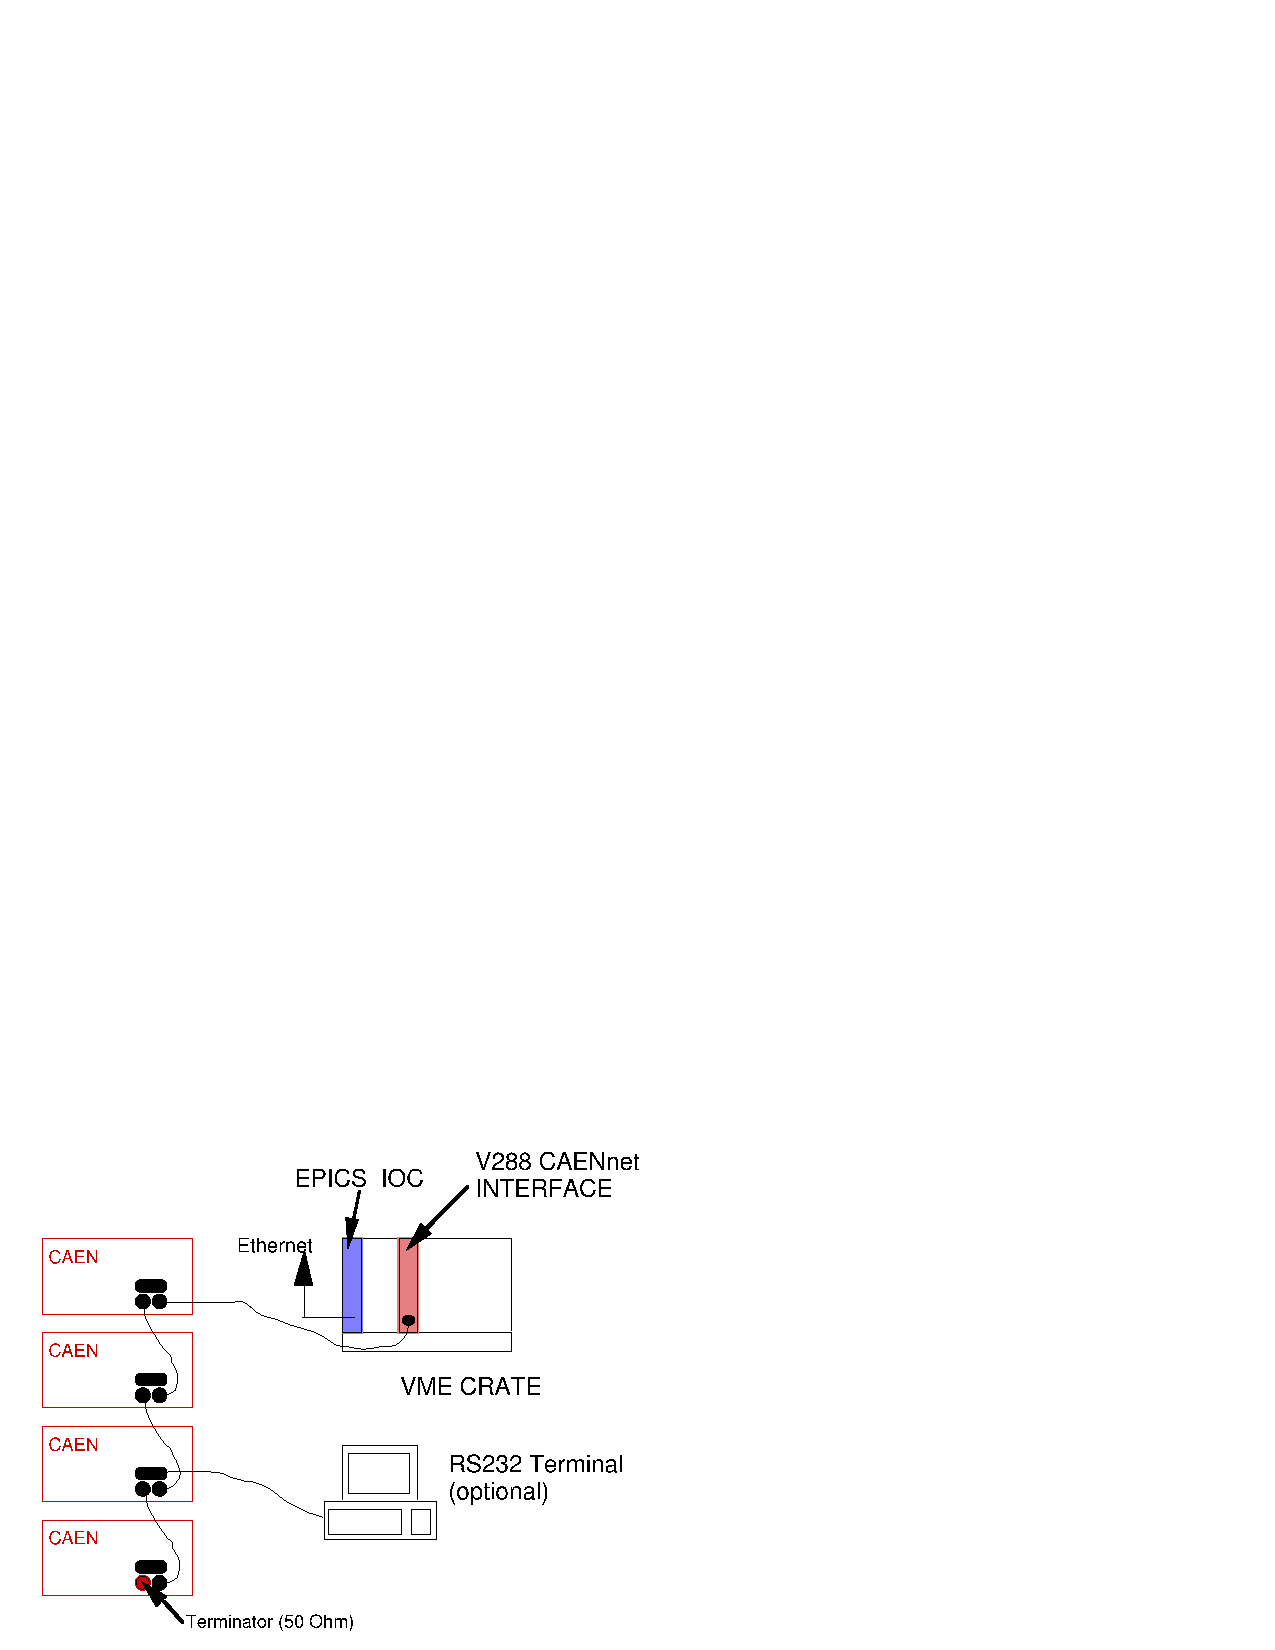
\includegraphics[height=4.5in]{CAENHV.pdf}
\caption{Generic CAEN High Voltage System setup\label{fig:caen_setup}}
\end{figure}

HV channel assignments currently in effect are indicated in 
two files ("group\_map" and
"channel\_map") in the directories \$EPHHV/perl (for HMS) and \$EPSHV/perl (for
SOS) when you are logged in as cvxwrks to one of the cdaq machines.

%\vfil\eject
\paragraph{General Operation}

\subparagraph{Normal Operation:}

In general the high voltage system will be controlled or monitored
from the counting house using the EPICS slow control system which will
be interfaced through a V288 card located in a VME crate in rack CH03B13
in the electronics room of the counting house
(see Figure~\ref{fig:caen_setup}).  It is also possible, but not recommended,
to control a CAEN crate using its front panel display or a terminal
if one is connected to the crate.
For EPICS control/monitoring all crates must be interconnected with 50
ohm (terminated) cable and all crates must be powered on whether they
will be in use or not.

Configuration of individual HV output channels is done through a
text file which is read in and downloaded when EPICS control is
configured. Step by step instructions for modifying this file and
reconfiguring the system are provided in the document
\htmladdnormallink{$\sim$cdaq/documents/slow\_controls/hvcntl.text}{http://www.jlab.org/Hall-C/document/slow_controls/hvcntl.text}. Do the HV rebuilds on cdaqs1 as cvxwrks.


It is imperative that
you follow the steps as shown there and not try to invent your own
procedure.
All relevant parameters
can be programmed through this interface.  The user must only know the
Crate Numbers and the Channel Numbers that his equipment is connected
to.  The crate number can be gotten from the front panel display and the
channel numbers run from 0-63 for each crate ( If only three cards are
installed, the channel number will run from 0-47 top to bottom
regardless of their positions in the crate).

\subparagraph{Important Features:}

The user can program several important features for individual
cards and/or channels.  The most common are:

\begin{itemize}
\item{HV limits -- 2 types including a hardware maximum (common to a
card) set with a pot on the front panel of each card and a software
maximum for each channel.}
\item{Current Trip Value -- The current over which the system will
indicate an alarm status and initiate a trip off of that channel.}
\item{Current Trip Time -- The amount of time the system will allow
the alarm condition before actually switching off that channel.}
\item{Ramp-up Value -- The number of volts/sec the voltage will ramp
to its set point upon switching on the channel.}
\item{Other Features -- See the CAEN Technical Information Manual.}
\end{itemize}

\subparagraph{Remote Operation: the High Voltage GUI system}
Remote operation of the CAEN system is described in the section
\ref{par:hv_ops}.

\subparagraph{Local (Front Panel) Operation}

Modifications to the parameter settings should in general not be
made at the front panel or through a locally connected terminal if the
EPICS system is in operation.  This mode of control is meant for
diagnostics and testing of a detector system prior to running.  There is
only one feature which must be set at the front panel before initiating
an EPICS control session - this is the crate number.  The RS232
parameters must also be set from the front panel ( suggested default are
9600 baud  no parity  1 stop bit).

If unfamiliar with the operation of the HV system in local modes
one should get experienced personnel or review the CAEN Technical
Information Manual.

\paragraph{Safety Concerns/Caveats}

There are a number of cautions one should observe when operating
the CAEN HV equipment to avoid damage and insure proper functioning:

\begin{itemize}
\item{Use only proper SHV connectors and approved cables when
connecting equipment to the supply.}
\item{{\bf DO NOT} attach/remove HV cables when loads are present on the
channel ( a red LED above each channel indicates the presence of a
load).}
\item{Insure adequate ventilation around crates to avoid overheating
of the electronics.}
\item{Wait 2-3 minutes after switching off a crate before removal of a
HV card.}
\item{Insure proper static precautions when handling HV cards.}
\end{itemize}

For proper EPICS control operation:

\begin{itemize}
\item{Inter-crate connections must be unbroken and terminated at the
last crate at 50 Ohms.  All crates must be powered on.}
\item{Crate numbers for each crate in the chain must be distinct and
different from 0 (i.e. 1-99)}
\item{The HV Enable switch (on the front panel of each crate) must be on.}
\item{One should refrain from any local operation of crates when the
EPICS system is active.}
\end{itemize}

\subsection{The Gas Mixing System}

The Hall~C On-line gas mixing system exists in the gas shed located
to the left of the counting house in the parking lot between the counting house
and the accelerator service building.
It provides two parallel
flow-controlled gas streams from a common source.  Flow rates, and gas mix
can be controlled independently in each of the gas streams.  The main
component of the system is a single MKS 647 menu driven 4-channel
controller that operates both of the parallel systems.  Gas flow is
controlled by 2259c proportional mass flow control valves.  The 647 allows
the Gas Calibration factor to be altered in software, allowing the user to
change to a different gas without recalibration of the mass flow control
valves.

A temperature controlled alcohol bubbler is provided for each gas
stream.  The alcohol level in each stream is maintained by a float valve
fed from a reservoir outside the bubbler chiller. This allows the alcohol
system to be refilled without opening the system to air.  A sight glass on
the side of the reservoir allows the level to be monitored.  A by-pass loop
around each alcohol system is provided should alcohol free gas be desired
or if the alcohol system requires maintenance.

The 647 is factory upgradeable to 8 channels.  The gas mixing
system has been plumbed to provide 2 parallel 3 channel gas streams.  In
the original installation, the mass flow control valves for channels 5 and
6 (gas \#3) were not installed.

To upgrade to 6 channel operation, 2 additional 2259c valves need
to purchased and installed.  The 647 needs to be returned to the factory
for the upgrade to 8 channel operation

The system will support a remote monitor and remote control through
a separate display port and an RS232 port on the back of the MKS 647 unit.

{\bf This system operates by measuring and controlling flow rate instead
of pressure. This system will maintain a constant rate of flow
regardless of pressure. It should not be used without appropriate pressure
relief device such as relief bubblers and relief valves. It should not be
connected to a closed vessel or system.}

{\bf Warning:} {\em{When using flow controlled systems such as this one, one 
must never introduce gas into a vessel without insuring that an outlet from the vessel is 
open.  The gas will continue to flow at the flow rate set point until the gas 
reaches the pressure setting of the pressure device ie. the regulator or relief 
bubbler, or until the vessel fails}.}

The manual valves used in this system are numbered on their
handles.  Those numbers are referenced in this document and in
Figure~\ref{fig:gas_mix}.
\begin{figure}
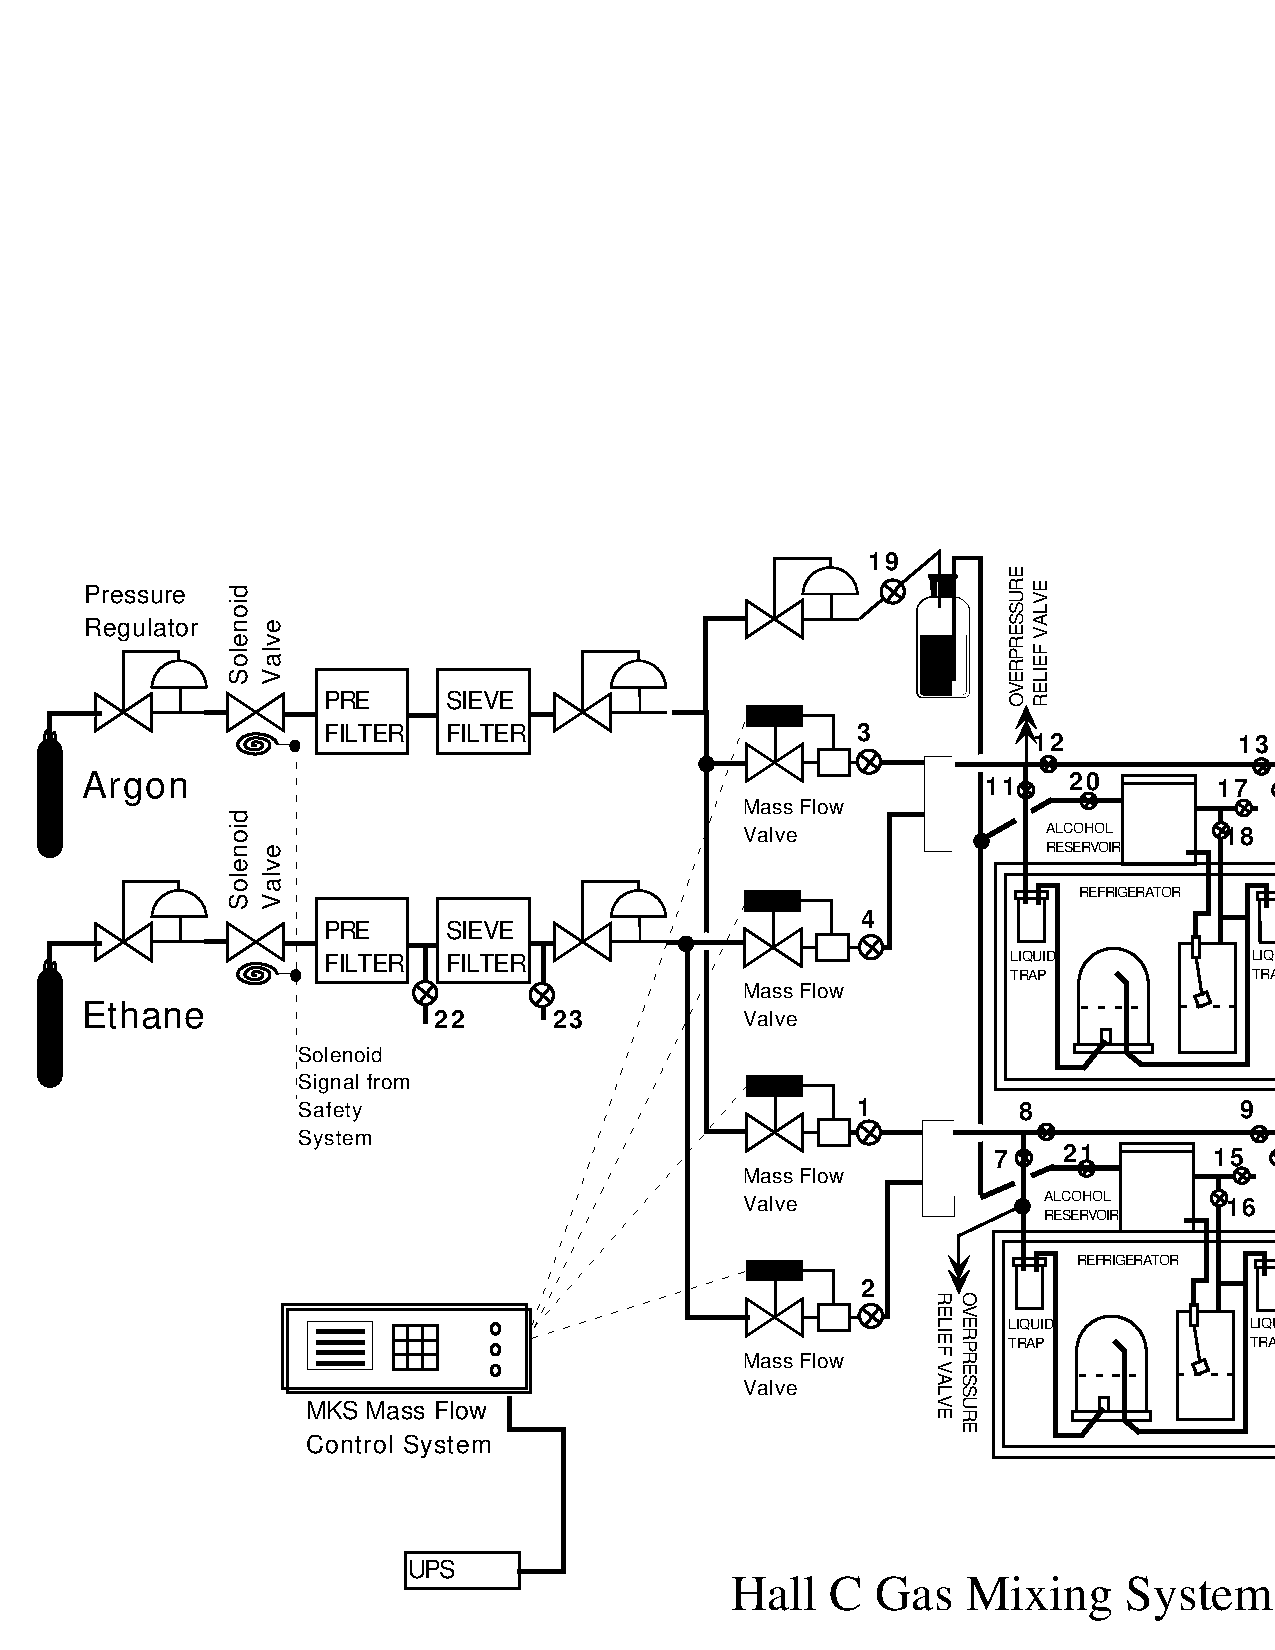
\includegraphics[width=6in,bb=12 12 750 590]{HallCGasMixlvl1.pdf}
\caption{Diagram of Hall~C Gas Mixing System\label{fig:gas_mix}}
\end{figure}

\paragraph{Normal Operation.}

For normal operation, with the alcohol systems in use, the following valves
should be set as follows:

{\bf For The HMS:}

Open - 3, 4, 11, 14; Closed - 12, 13, 17, 18, 19, 20


Unless the gas \#3 Mass flow control valve is installed, valve \#6 should
always be closed.

{\bf For the SOS:}

Open - 1, 2, 7, 10; Closed - 8, 9, 15, 16, 19, 21.


Unless the gas \#3 Mass flow  control valve is installed, valve \#5 should
always be closed.

\paragraph{Operating the MKS 647 Mass Flow Controller.}

The gas flow is controlled by a MKS 647 controller and mass flow
control valves.  The 647 is menu driven from a CRT in the front panel and
with a keypad with cursor controls. The 647 features a non-volatile memory
so settings are retained even if the unit is unpowered.  The initial menu
upon startup is the Command Menu.  For normal operation use either the User
Display menu (Command menu item \#1) or the Extended Display menu (Command
menu item \#2).  The User Display menu shows actual flow in each channel and
the total flow in all channels.  The Extended Display menu shows actual
flow, flow set point, units, valve full scale range, gas calibration
factor, whether that channel is enabled, and whether each channel is
operating in master, slave, or independent mode.

{\bf To set flow rates:}

The flow rate set points are adjusted from the Extended Display
menu.  There are two methods to change valve flow rate set point.  If you
want to enter a specific value you must first turn off the flow in that
channel or all of the channels.  Using the cursor keys move the cursor to
the desired channel.  Enter the desired flow rate.

The flow rate set point can be changed with gas flowing using the
cursor keys. In the Extended Display mode move the cursor to the desired
channel using the left/right cursor keys.  The set point can then be
adjusted up or down using the cursor up/down keys.

{\bf To turn gas flow on or off:}

The gas flow can be turned on or off while in any menu.  When any
of the mass flow valves are open the green LED labeled ``GAS ON" on the 647
is lit.  When none of the gas flow valves are open the red ``STAND BY" LED
will be flashing.  In the Extended Display menu the bottom line displays on
or off, by channel, to show which mass flow valves are enabled.  The green
LED must be lit and an ``ON" must be displayed in the bottom row of the
Extended Display menu for gas to be flowing in a particular channel.

{\bf Turning the gas on or off is done in two steps which can be done in
either order.}
Each channel must be enabled by pressing ``ON" and then
that channel number.  The command input must be enabled by pressing ``ON"
and then ``ALL" from the keypad.  This allows a single channel or all of the
enabled channels to be turned on or off at once.  Both steps must be
performed initially, but thereafter only one of the steps need be performed
to cycle the gas flow on or off.

To turn gas off in a single channel press ``OFF" and then the
desired channel.  If you want to close all the valves simultaneously, press
the ``OFF" key and then the ``ALL/0" key.  To turn gas back on you must
reverse whichever sequence you used to stop the gas flow.  For example if
you turned the gas off by pressing ``OFF" and then the channel number, it
must be turned back on by pressing ``on" and then the channel number.  If
you turn off all the channels by pressing ``OFF" , ``ALL" you must turn it
back on by pressing ``ON" , ``ALL."

{\bf To by-pass the alcohol system:}

For the HMS:
Open valves 12 \& 13, then close valves 11 \& 14, in that order!

For the SOS:
Open valves 8 \& 9, then close valves 7 \& 10, in that order!

{\bf To refill the alcohol bubblers:}

The alcohol bubbler system features a refill system that allows
filling directly from the bottle, minimizing exposure of the alcohol to air
and reducing the possibility of a spill.
{\bf The reservoirs should be refilled
before they become empty to maintain a head of liquid over the float valve
which will prevent air from entering the system.}
In the back of the gas
system rack is a holder for gallon sized alcohol bottles and a cap with dip
tube.  Place a new bottle in the bottle holder and replace the cap with the
cap with dip tube.

\begin{itemize}
\item{ \bf{Step-by-Step Instructions for Refilling the SOS Alcohol Bubbler}\\
\em{These steps must be individually completed in the order listed!}}\\
Refer to Fig.~\ref{fig:gas_mix}. 
\begin{enumerate}
\item{If needed, install a full bottle of alcohol in the back of the gas racks as mentioned in the preceeding paragraph.}
\item{{\em Open valves 8,9. Close valves 7,10} to Put the SOS alcohol bubbler in BYPASS.}
\item{{\em Close valve 16} to isolate the warm reservoir gas from the bubbler.}
\item{{\em Open valve 15} to bleed off the warm reservoir gas pressure.}
\item{{\em Open valve 19} to pressurize the alcohol bottle.}
\item{{\em Open valve 21} to flow alcohol into the warm reservoir.}
\item{When the alcohol level in the sight-glass is within 2cm of the top, stop
the flow of alcohol: {\em Close valve 21.}}
\item{{\em Close valve 19.}}
\item{{\em Open valve 16.}}
\item{{\em Close valve 15.}}
\item{{\em Open Valves 7 and 10. Close Valves 8 and 9.}}
\item{Record what you did in both the gas logbook and the electronic logbook.} 
\end{enumerate}

\item{ \bf{Step-by-Step Instructions for Refilling the HMS Alcohol Bubbler}\\
\em{These steps must be individually completed in the order listed!}}\\
Refer to Fig.~\ref{fig:gas_mix}. 
\begin{enumerate}
\item{If needed, install a full bottle of alcohol in the back of the gas racks as mentioned in the preceeding paragraph.}
\item{ {\em Open valves 12,13. Close valves 11,14} to Put the HMS alcohol bubbler in BYPASS.}
\item{{\em Close valve 18} to isolate the warm reservoir gas from the bubbler.}
\item{{\em Open valve 17} to bleed off the warm reservoir gas pressure.}
\item{{\em Open valve 19} to pressurize the alcohol bottle.}
\item{{\em Open valve 20} to flow alcohol into the warm reservoir.}
\item{When the alcohol level in the sight-glass is within 2cm of the top, stop
the flow of alcohol: {\em Close valve 20.}}
\item{{\em Close valve 19.}}
\item{{\em Open valve 18.}}
\item{{\em Close valve 17.}}
\item{{\em Open Valves 11 and 14. Close Valves 12 and 13.}}
\item{Record what you did in both the gas logbook and the electronic logbook.} 
\end{enumerate}
\end{itemize}

\paragraph{Recalibration and Rezeroing}

Mass flow control valves(the 2259c's) require periodic recalibration
and rezeroing.

\noindent{\bf Rezeroing:}

Rezeroing or Zero Offset is easy and can be performed often and should be
performed every time the unit is moved, recalibrated, or adjusted.  The
valve must be in the orientation it will be used to rezero it.
{\bf To use the
Auto Zero function one must insure that the channel is not switched on and
there is no possibility of flow in that channel ie. the manual valve in
line with the mass flow valve must be closed.}
The Zero Adjust menu is
reached from the main menu to the Instrument Setup menu.  In the Zero
Adjust menu move the cursor to the word EXEC on the channel to be zeroed in
Zero Adjust line.  The unit will measure the current value and use that for
the new zero offset.  If the operation is successful the word EXEC will be
changed to Done.  If the offset is too large or that channel is on, the
unit will display fail.  In that case, one should check if there is any
flow (even extremely small flow) through the valve.

\noindent{\bf Recalibration:}

MKS recommends recalibration every 12-24 months.  The valves must be
returned to the factory for recalibration.  After reinstallation, the
valves need to be rezeroed.

\paragraph{Filtering}

{\bf All filter maintenance should be performed with the gas supplies shut off
at the tanks.  Insure that no pressure remains inside the filter
before proceeding.}

Both input channels of this system feature high performance long life
filters using a pre-filter and molecular sieve in stainless steel filter
vessels.  The pre-filter and filter cartridges are available from the
company listed below.  The pre-filter is a mechanical filter to remove
liquids and solids from the gas stream and to protect the molecular sieve
downstream from it.

\noindent{\bf Replacing filter cartridges:}

The cartridges are replaced by loosening the nut on the bottom of the bowl
and removing the bowl.  The cartridges can be exchanged and the bowl and
nut replaced and tightened.

\noindent{\bf Using 13x molecular sieve filters with ethane:}

{\sl It has been reported that when using 13x molecular sieve filters with
ethane, some ethane is trapped in the filter making the cartridges
flammable.   To purge the ethane from the  filter cartridge a pair valves
and external connections are on either side of that cartridge.  A nitrogen
line should be connected to valve \#22 and a vent line connected to valve
\#23 before changing filters. Nitrogen should flow through the filter for
several hours before changing.}

\noindent {\bf Purchasing Filters and Repairs:}

The following filter types are used:
\begin{itemize}
\item[~]3/100-12-bx microfiber pre-filter
\item[~]CI-100-12-103 molecular sieve final filter
\end{itemize}

These filter cartridges are available from:  Balston Filters, 6767 Forest Hills Drive, Suite 305, Richmond, VA 23225,  1-800-221-1900

Recalibration and repair of the mass flow control valves and controller are
available from:  MKS instruments, Six Shattuck Road, Andover, MA 01810,  
1-800-227-8766 or508-975-2350



\subsection{Hall C Laser Pulser System}
The Hall C laser pulser sytem provides light pulses
in the visible  blue scintillation region to monitor
the gain stability of the HMS and SOS shower counters and scintillators,
and, at a later stage, the neutron detector of the $G_{En}$ experiment.

\paragraph{UV Laser System}
We use a nitrogen Laser that provides UV laser pulses at 337 nm
from 1 to 50 Hz repetition rate. The output power is 250 $\mu$J.
It is located in a designated area in the Counting House of Hall C.
The laser is enclosed in an aluminum box where the laser light is directed
onto a scintillation fiber after passing through two optical filters
to optimize the light output. 
The laser light is absorbed in the scintillation fiber
and converted to visible blue scintillation light. Both ends of the
scintillation fiber are coupled using CT connectors, mounted on an
aluminum casing, to regular
1 mm diameter multimode plastic optical fibers. One fiber output is
connected to a PIN diode to monitor the light output; the other
fiber is brought downstairs into Hall C where it is connected to 
a distribution box (1:24) located in the cupboard below the pivot. From
this distribution box 4 fibers are running to the HMS spectrometer and
4 to the SOS spectrometer, where they
are connected again to distribution boxes (1:64). The individual
outputs of the final distribution box are connected to the scintillators
and lead glass shower counters. The light pulses in the detector
produce a trigger in the data acquisition system and ADC and TDC
information is read out. Normalizing the peak positions of the light 
pulses to the PIN diode ADC value is a tool to monitor the gain of
each photo multiplier tube throughout the experiments.

\paragraph{Laser Operation} 
In order to turn on the nitrogen laser the right half of the top
plate of the aluminum box needs to be removed. Inside the box 
the laser and the optics is mounted on a single aluminum board.
The lasing part of the laser is confined in the left part of the box
with a separation in the central region of the box. Due to this separation
no UV laser light can escape from this left part of the box,
even during operation, so that the user can safely remove and install the
top plate above the right half of the laser casing.
The laser itself has a security key that needs 
to be in a vertical position when the power switch is pressed. After
2 minutes of warmup-time an orange light turns on indicating that
it is possible now to turn the key into its horizontal position.
After this it takes 15 seconds until the laser actually turns on.
In the event of a power failure the laser will turn off and will not
turn on again after power is restored. It is necessary to turn the key
back to its vertical position and to reset the safety system of the laser.
The laser can now be turned on again by switching the key back to its
horizontal position. The pulse frequency of the laser can be regulated by
turning the black knob at the rear of the laser casing.
